\begin{exsol}{4}{\MG{} Ch.~1, Exercise 5}{8}{Foundations}{B1}
\asked (a) Draw the prisoners' dilemma of Fig.~1.8 (pp.~8--9) as a game tree; (b) mark the
initial node, the terminal nodes and the information set, and explain why the information set is
there; (c) count each player's strategies.

\method Extensive form with an information set for simultaneous moves (Lecture~1, slides~15
and~17; Tadelis \S3.1); dominance and Pareto optimality (slides~23--26).

\solution
Payoffs are minus the years in jail: $C$ = confess, $N$ = not confess.
\begin{center}
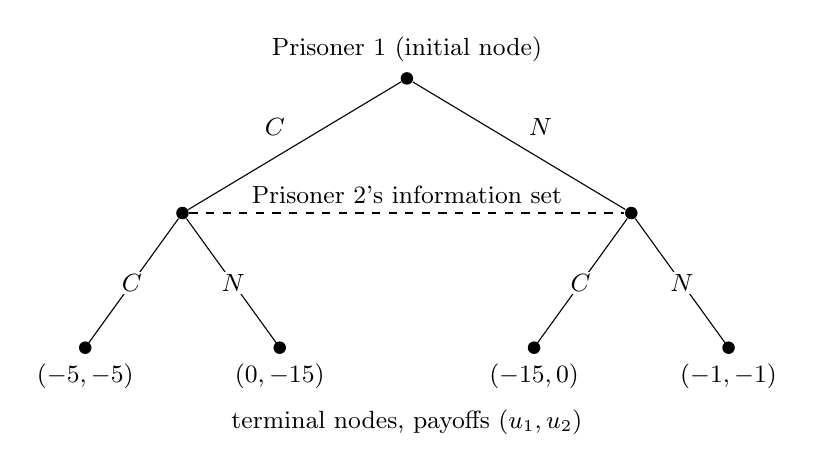
\begin{tikzpicture}[scale=0.95,
  dot/.style={circle,fill,inner sep=1.6pt}, every node/.style={font=\small}]
  \node[dot,label=above:{Prisoner 1 (initial node)}] (r) at (0,0) {};
  \node[dot] (a) at (-3,-1.8) {};
  \node[dot] (b) at (3,-1.8) {};
  \draw (r) -- node[above left] {$C$} (a);
  \draw (r) -- node[above right] {$N$} (b);
  \draw[dashed] (a) -- node[above] {Prisoner 2's information set} (b);
  \foreach \x/\p/\lab/\pay in {-4.3/a/$C$/{$(-5,-5)$}, -1.7/a/$N$/{$(0,-15)$},
                               1.7/b/$C$/{$(-15,0)$}, 4.3/b/$N$/{$(-1,-1)$}} {
    \node[dot,label=below:{\pay}] at (\x,-3.6) {};
    \draw (\p) -- node[fill=white,inner sep=1pt] {\lab} (\x,-3.6);
  }
  \node at (0,-4.6) {terminal nodes, payoffs $(u_1, u_2)$};
\end{tikzpicture}
\end{center}

\textbf{(b)} The initial node (root) is player~1's decision. The four terminal nodes carry the
payoffs. The dashed line joins player~2's two decision nodes into one \emph{information set}:
she does not know which node she is at, because she decides without observing player~1's choice.
This is how a tree represents simultaneous moves; drawing player~2 first instead gives the same
game.

\textbf{(c)} A strategy assigns an action to each information set. Player~1 has one, player~2
has one (not two), so $S_1 = S_2 = \{C, N\}$: two strategies each. Without the dashed line
player~2 would have $2^2 = 4$ strategies, as in item~3.

\textbf{Dominance and Pareto (the lecture's lessons).} For each prisoner, $C$ strictly dominates
$N$: $-5 > -15$ against $C$ and $0 > -1$ against $N$. So $(C,C)$ is the strict dominant-strategy
equilibrium, and by slide~29 the unique IESDS survivor. But $(N,N)$ gives $(-1,-1)$, better for
both than $(-5,-5)$: the equilibrium is not Pareto optimal (slides~25--26, Lessons~1 and~2).

\interp The information set encodes what a player knows when moving, and therefore what her
strategies can depend on. In the dilemma, individually rational choices waste five years each.

\verify \texttt{check\_A.py} checks that $C$ strictly dominates $N$ for both players, that
IESDS leaves only $(C,C)$, and that $(N,N)$ Pareto-dominates it. The book's answer (p.~10)
agrees on (a)--(c); the dominance paragraph goes beyond it.

\answer{Tree above: root = prisoner~1's choice, four terminal nodes with payoffs $(-5,-5)$,
$(0,-15)$, $(-15,0)$, $(-1,-1)$, and one information set joining prisoner~2's nodes because she
cannot observe prisoner~1. Each player has two strategies, $\{C, N\}$. Confess is strictly
dominant; $(C,C)$ is Pareto-dominated by $(N,N)$.}
\end{exsol}
